%%%%%%%%%%%%%%%%%%%%%%%%%%%%%%%%%%%%%%%%%%%%%%%%%%%%%%%%%%%%%%%%%%%%%%%%%%%%%%%
%                          LaTeX beamer template                              %
%              © 2010 Valentin Roussellet (louen_AD_palouf.org)               %
%    Distributed under the terms of WTFPL v2, see http://sam.zoy.org/wtfpl    %
%%%%%%%%%%%%%%%%%%%%%%%%%%%%%%%%%%%%%%%%%%%%%%%%%%%%%%%%%%%%%%%%%%%%%%%%%%%%%%%
\documentclass{beamer}
% A reminder for beamer themes and colors
%                       Themes
% -----------------------------------------------------------------------------
% * Warsaw : black / colored toc above. Most commoly used
% * Copenhagen : like Warsaw without shadows
% * Marburg : black to blue right-sided toc
% * Berlin : colored panels above the text
% * Antibes : a lot like berlin
% * PaloAlto : colored left-sided toc
%                       Colors
%------------------------------------------------------------------------------
%   Name               background       titles          text
% * orchid (default)   white            dark blue       black
% * albatross          blue             light blue      white
% * beetle             grey             white           black
% * crane              white            black/yellow    black
% ============================== PREAMBLE =====================================
% Beamer settings ----------------
\mode<presentation>{
  %\usetheme{Marburg}                            % theme (see above)
  \usetheme{PaloAlto}                            % theme (see above)
  \usecolortheme{crane}                        % theme color (id)
  \setbeamercovered{transparent}                % For transparent zones
}

% Encoding and fonts -------------
\usepackage[utf8]{inputenc}                     % Input encoding
\usepackage[T1]{fontenc}                        % Output encoding
\usepackage{lmodern}                            % Modern font

% Language -----------------------
%\usepackage[right]{eurosym}                     % Symbol for euro
%\usepackage[french]{babel}

% Useful packages ----------------
\usepackage{listings}                           % for source code inclusion
\usepackage{hyperref}
\hypersetup{linkcolor=cyan}

% Mathematical symbols------------
\usepackage{amsmath}
\usepackage{amsfonts}
\usepackage{amssymb}

% Custom colors -----------------
\definecolor{codebg}{rgb}{0.97,0.97,0.97}
\definecolor{codecomment}{rgb}{0,0.5,0}
\definecolor{codestring}{rgb}{0.5,0,0}

% Listings setup -----------------
\lstset{language=C++,                             % programming language
%morekeywords={},                                % additionnal keywords
basicstyle=\small\ttfamily,                     % style of the code
keywordstyle=\color{blue}\bfseries,             % style of the keywords
stringstyle=\color{codestring},                 % style of the strings
commentstyle=\color{codecomment},               % style of the comments
showspaces=false,                               % do not underline spaces in code
showstringspaces=false,                         % do not underline spaces in strings
showtabs=false,                                 % do not underline tabs
numbers=left,                                   % where are the line-numbers
numberstyle=\tiny,                               % style of the line-numbers
backgroundcolor=\color{codebg},                 % background-color
stepnumber=1,                                   % the step between two line-numbers.
extendedchars=true,                             % allows extended characters
columns=flexible,                               % sets the columns to non-fixed width
tabsize=2,                                      % sets the tabulation width
frame=trBL,                                     % adds a frame around the code with double line on the bottom
frameround=tttt,                                % rounds the frame
breaklines=true,                                % line breaks automatically
breakautoindent=true,                           % keep indentation level withh line breaks
captionpos=b                                    % the caption is at the bottom
}

% Additional beamer commands ------
% this command prints a frame toc at each section beginning
% \AtBeginSection[] {
%   \begin{frame}
%       \frametitle{What next ?}
%       \tiny{\tableofcontents[currentsection]}
%   \end{frame}
% }

% ============================== FRONT MATTER =================================
\title{}
\subtitle{}
\author{Charly \textsc{Mourglia} \& Valentin \textsc{Roussellet}}
\institute[IRIT]{IRIT}
\date{\today}
\subject{}                                      % Information PDF
%\logo{\includegraphics[height=1cm]{logo.png}}  % Logo

% ============================= END OF PREAMBLE ===============================
\begin{document}
\begin{frame}
  \titlepage
\begin{center}
\href{mailto:valentin.roussellet@irit.fr}{valentin.roussellet@irit.fr}
\end{center}
\end{frame}

\section{Constraints}
\begin{frame}
 \frametitle{What are constraints ?}
 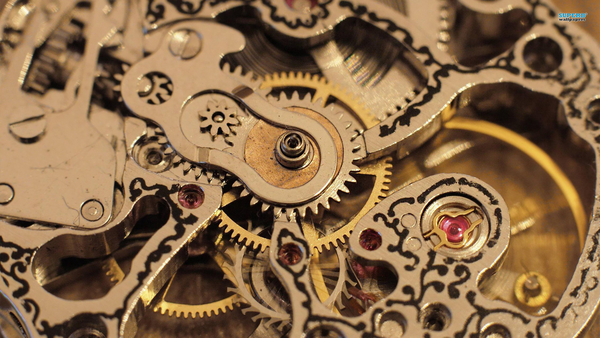
\includegraphics[width=\textwidth]{watch.png}\\
  Joints, contacts, mechanical links...
\end{frame}

\begin{frame}
\frametitle {Real-life examples}
\begin{center}
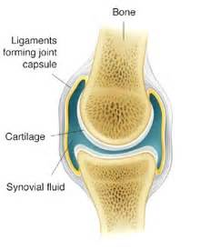
\includegraphics[width = 0.2\textwidth]{humanjoint.png}
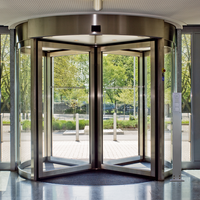
\includegraphics[width = 0.2\textwidth]{door.png}
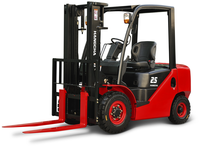
\includegraphics[width = 0.2\textwidth]{elevator.png}
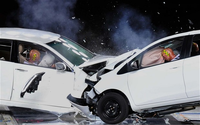
\includegraphics[width = 0.2\textwidth]{carcrash.png}
   \begin{exampleblock}{Examples}
    \begin{center}
     \begin{tabular}{c c c c}
       Human joint & Revolving door & Elevator & Collision \\
       Ball-socket & Hinge & Slider & Non-penetration
     \end{tabular}
     \end{center}
   \end{exampleblock}
   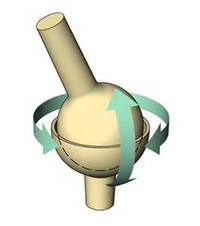
\includegraphics[width = 0.2\textwidth]{ballsock.png}
   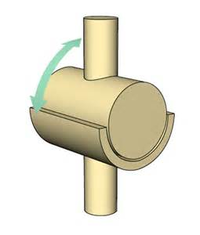
\includegraphics[width = 0.2\textwidth]{hinge.png}
   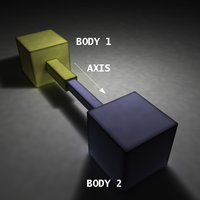
\includegraphics[width = 0.2\textwidth]{slider.png}
   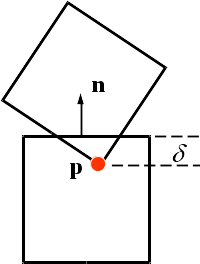
\includegraphics[width = 0.2\textwidth]{collision.png}
\end{center}
\end{frame}
\subsection{Modeling constraints}
\begin{frame}
 \frametitle{What are constraints ?}
 \begin{block}{Constraints}
  \begin{itemize}
    \item A constraint limits \textbf{degrees of freedom} of rigid bodies. \pause
    % NOTE : 2 RBs have 2 * 6 = 12 DOF.
    \item Engine computes \textbf{constraint forces} to apply to the bodies.
    \item Constraints must be \textbf{solved} by the physics engine to be satisfied.
  \end{itemize}
  \end{block}
\end{frame}


\begin{frame}
 \frametitle{Here comes the physics}
 \begin{itemize}
  \item A constraint can be written as an equation $C(\mathbf{q}) = 0$
  \item Example : Ball-socket $\mathbf{c_1} + \mathbf{r_1} - (\mathbf{c_2} + \mathbf{r_2}) = 0$\\
  \begin{center}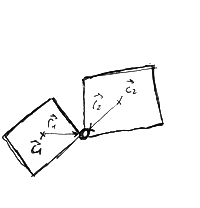
\includegraphics[width = 0.4\textwidth]{jacobian1.png}\end{center}
  \pause
  \item We can derive and get a velocity equation $\dot{C} = 0$.
  \item $\mathbf{v_1} + (\mathbf{\omega_1} \times \mathbf{r_1}) - ( \mathbf{v_2} + (\mathbf{\omega_2} \times \mathbf{r_2})) = 0$
  \end{itemize}
\end{frame}

\begin{frame}
 \frametitle{Jacobians}
 \begin{block}{Jacobian : definition}
 \begin{itemize}
  \item Velocities constraints can be written as a scalar product
  \item $J\mathbf{v} = 0$
  \pause
  \item Virtual work theorem : $\mathbf{F_c} = J^T \mathbf{\lambda}$
  \end{itemize}
  \end{block}
\end{frame}

\begin{frame}
 \frametitle{Jacobians : the dirty details}
  \begin{center}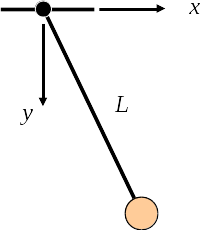
\includegraphics[width = 0.2\textwidth]{pendulum.png}\end{center}
  \begin{itemize}
    \item $C(x,y) = x^2 + y^2 - L^2 = 0$
    \pause
    \item $\frac{\mathrm{d}C}{\mathrm{d}t} = \frac{ 1 }{\sqrt{x^2+y^2}} \begin{pmatrix} x & y\end{pmatrix} \begin{pmatrix} v_x \\ v_y\end{pmatrix}$
    \pause
    \item VWT : $\mathbf{F_c} = \lambda \begin{pmatrix}x\\y\end{pmatrix}$ 
  \end{itemize}
  How do we compute $\lambda$ ?
\end{frame}

\subsection{Physics solver}

\begin{frame}
 \frametitle{What is the solver doing ?}
 \begin{block}{Solver Algorithm}
 \begin{enumerate}
  \item Apply external impulses (e.g. gravity) $\bar{\mathbf{v}} = \mathbf{v} + M^{-1} \mathbf{P_{ext}}$
  \item Apply constraint impulses by solving for all $\lambda$
  \item Update positions from velocity.
 \end{enumerate}
 \end{block}
 Reminder :
 \begin{description}
    \item[Impulse] $\mathbf{P} = \mathbf{F} \delta t$
    \item[Newton] $\delta \mathbf{v} = M^{-1} \mathbf{P}$
 \end{description}
\end{frame}

\begin{frame}
 \frametitle{Finding $\lambda$}
  \begin{description}
   \item[Newton] $\mathbf{v'} = \bar{\mathbf{v}} + M^{-1} \mathbf{P_{c}}$
   \item[VWT] $\mathbf{P_c} = J^T \lambda$
   \item[Constraint] $J\mathbf{v'} = 0$
  \end{description}  
  \pause
  \begin{block}{Solution}
   \[ \lambda = -m_c (J \bar{\mathbf{v}})\]
   \[ m_c = \frac{1}{J M^{-1}J^T} \]
   $m_c$ is the virtual mass seen from the constraint
  \end{block}
\end{frame}

\begin{frame}[fragile]
 \frametitle{Solving all bodies}
  \begin{itemize}
   \item All the $\lambda_{i,j}$ equations = one big very sparse linear system.
   \pause
   \item We could solve it globally (slow)
   \pause
   \item Instead iterative methods are used.
  \end{itemize}
  \begin{lstlisting}
while (abs(vNext - vCurrent) > epsilon) {
 for (auto c : constraint) {
   solve(c, lambda);
  }
}
  \end{lstlisting}
\end{frame}


\begin{frame}
 \frametitle{Extensions}
 \begin{minipage}{0.78\linewidth}
  \begin{itemize}
   \item \textbf{Inequality constraint} ($C(\mathbf{q}) \geq 0$) for contacts.
   \item \textbf{Bias} in constraint ($J\mathbf{v} + b = 0$)
   \pause
   \item \textbf{Baumgarte stabilization} to avoid position drift.
  \end{itemize}
 \end{minipage}
% \vspace{}
 \begin{minipage}{0.2\linewidth}
   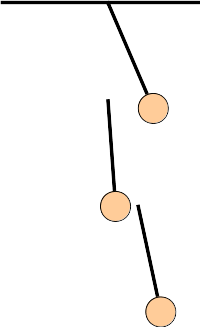
\includegraphics[width=0.9\textwidth]{blowup.png}
 \end{minipage}

\end{frame}


\begin{frame}
 \frametitle{Bibliography} 
  \begin{thebibliography}{9}
  \bibitem{Catto07} Erin \textsc{Catto} (Blizzard), \emph{Modeling and solving constraints}, Proceedings of GDC 2007.\href{http://box2d.org/files/GDC2007/GDC2007_Catto_Erin_Physics1.ppt}{[PPT]} 
  \bibitem{Catto07} Erin \textsc{Catto} (Blizzard), \emph{Computing Distance using GJK}, Proceedings of GDC 2010. \href{http://box2d.org/files/GDC2010/GDC2010_Catto_Erin_GJK.pdf}{[PDF]}
  \bibitem{Ericson04} Christer \textsc{Ericson} (Sony), \emph{Real-time collision detection}. CRC Press, 2004.
  \bibitem{Shabana09} Ahmed A. \textsc{Shabana} (U.Illinois), \emph{Computational dynamics}. John Wiley \& Sons, 2009
  \end{thebibliography}
\end{frame}


\end{document}
